%%%%%%%%%%%%%%%%%%%%%%%%%%%%%%%%%%%%%%%%%%%%%%%%%
% Chapter: Events
%%%%%%%%%%%%%%%%%%%%%%%%%%%%%%%%%%%%%%%%%%%%%%%%%
\chapter{Event Notification}
\label{chap:api_event}

% RALPH
\ldots


%%%%%%%%%%%%%%%%%%%%%%%%%%%%%%%%%%%%%%%%%%%%%%
%%%%%%%%%%%%%%%%%%%%%%%%%%%%%%%%%%%%%%%%%%%%%%
\section{Logging}
\label{chap:api_event:logging}

\par
The \refapi{PMIx_Log} interface is provided to support posting information by applications and \ac{SMS} elements to persistent storage. This function is \emph{not} intended for output of computational results, streaming of raw \ac{RAS} data, or performant data operations, but rather on reporting status and saving state information (e.g., inserting computation progress reports into the application's \ac{SMS} job log). A variety of logging options are available to support use-cases such as remote monitoring of application progress (e.g., via email), output of error reports to syslog for post-mortem analysis, and caching of application completion information for use by subsequent applications in a workflow. Depending on the choice of output channel, logged information may be retrievable via the \refapi{PMIx_Query_info_nb} interface.

\par
The illustration below highlights some of the capabilities provided by the logging support. Note that the illustration is not intended to be comprehensive in its coverage as the number of possible use-cases is too large to capture in a single drawing.

\begin{figure*}[ht!]
\begin{center}
  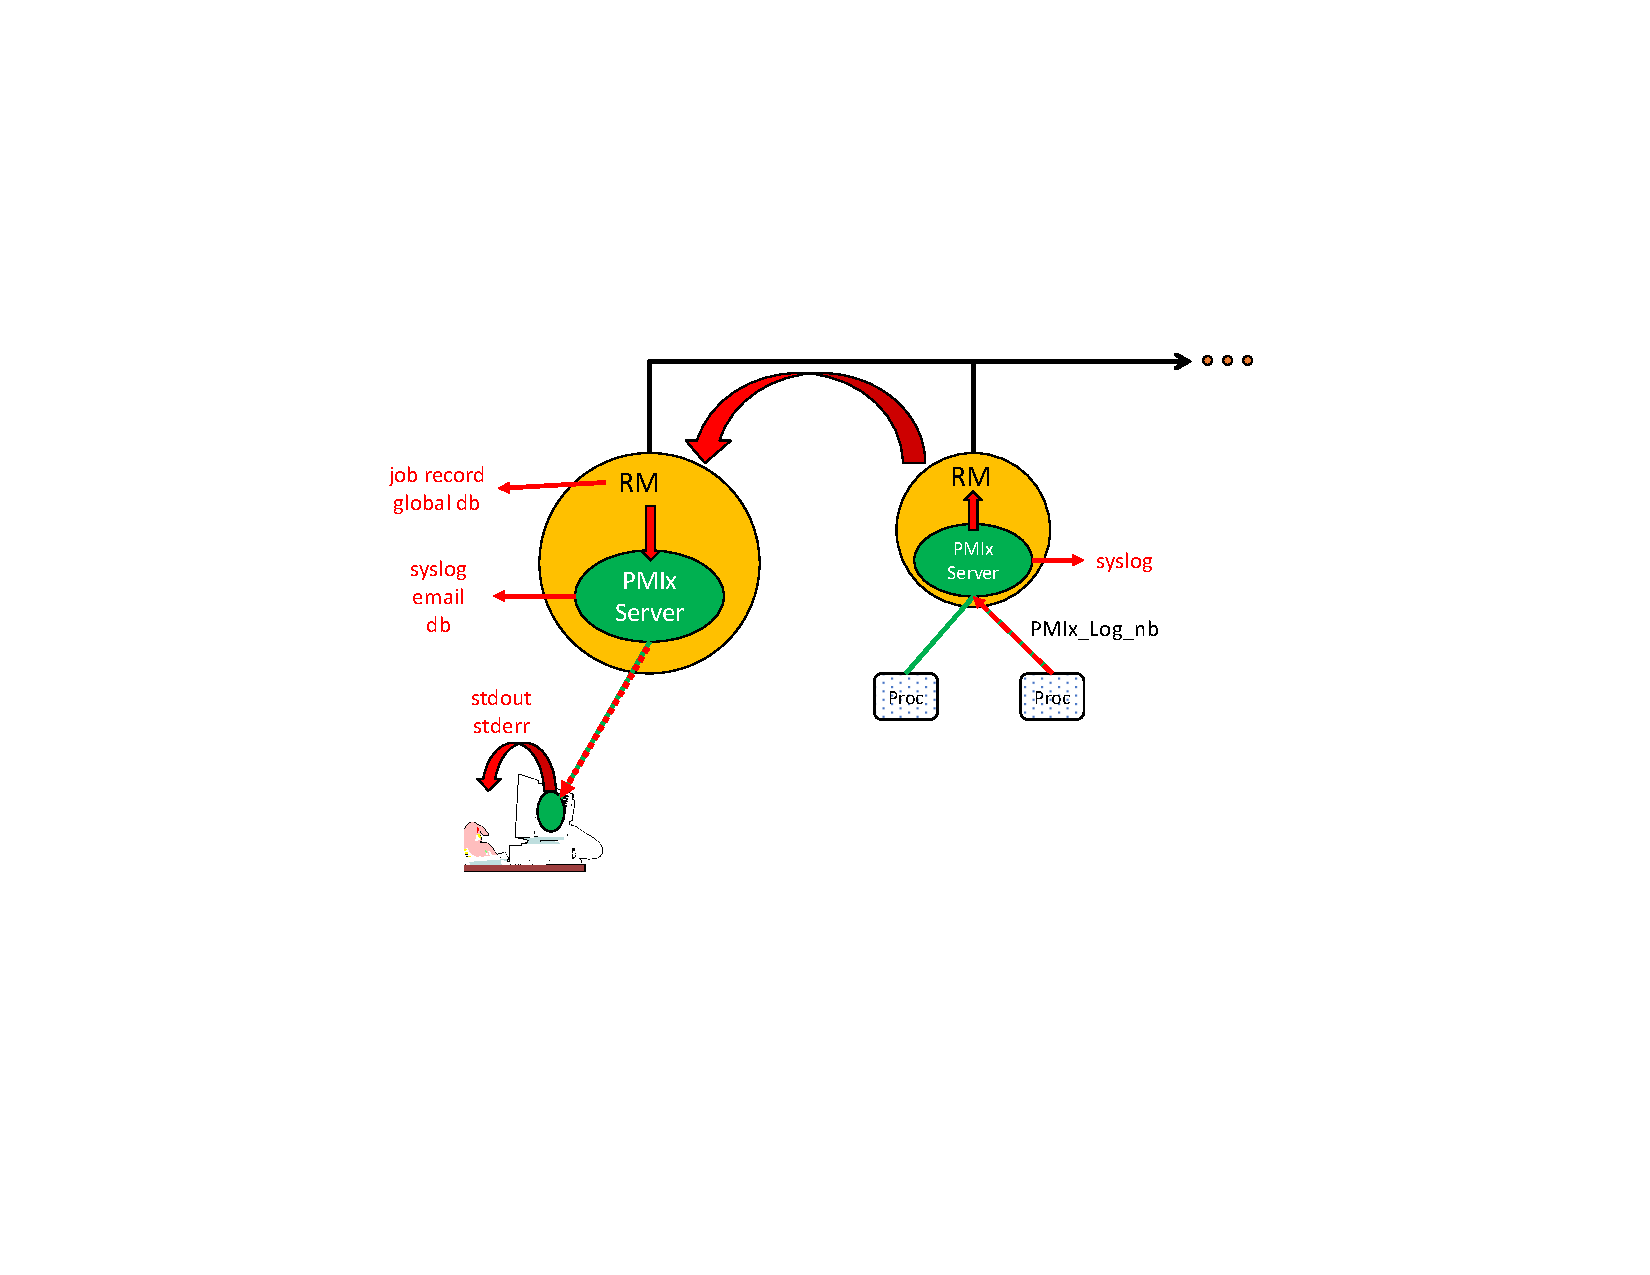
\includegraphics[clip,width=0.6\textwidth]{figs/logging.pdf}
\end{center}
  \caption{PMIx-based Logging}
  \label{fig:logging}
\end{figure*}



\par
Supported uses include:

\begin{itemize}
\item Writing of messages to syslog, both local (using the \refattr{PMIX_LOG_LOCAL_SYSLOG} attribute) or on the syslog of some central server designated for this purpose. The \ac{PMIx} client will send the logging request to its local server. If the \refattr{PMIX_LOG_LOCAL_SYSLOG} attribute is included in the request, then the \ac{PMIx} server will immediately output the message to the local syslog. If not, or if the \refattr{PMIX_LOG_GLOBAL_SYSLOG} attribute is specified, then the \ac{PMIx} server will forward the request to its host \ac{SMS} daemon. It is the responsibility of the host daemon to identify and transfer the provided data to the appropriate location --- upon arrival, the receiving daemon can use the \refapi{PMIx_Log} function to deliver the data to the local syslog on that node or can write the data to syslog itself. Attributes for setting the desired syslog priority are provided --- the default is set to to syslog priority LOG_INFO indicating reporting of an informational message

\item Sending notifications to a designated user. Application users may wish to be notified of completion of their application, receive periodic progress reports, or be notified of a problem that merits attention. \ac{PRI} includes support for some of the more popular transports --- requests for unsupported transports are referred to the host \ac{SMS} for processing, with an error returned if the requested transport is not available in the host environment

\item Outputting tagged log messages to stdout or stderr of the application, or a connected tool. Where supported, an alternative output stream (possibly directed to a dedicated log file) may be specified. Messages may be tagged (via the \refattr{PMIX_LOG_TAG_OUTPUT} attribute) as flowing via the \refattr{PMIx_Log} \ac{API} to differentiate them from the application's normal output. In addition, messages may be timestamped (\refattr{PMIX_LOG_TIMESTAMP_OUTPUT}) or output in \ac{XML} format (\refattr{PMIX_LOG_XML_OUTPUT})

\item Storing status updates in the job record using the \refattr{PMIX_LOG_JOB_RECORD} attribute. Resource managers nearly always maintain a record of the jobs they schedule and execute. This includes information on the time spent waiting for allocation, priority of the request, identity of the requestor, name/path of the executable and/or job script, etc. Historically, users have had to record status information on their application (e.g., computational progress) in files which are subsequently stored in persistent storage. \refapi{PMIx_Log} offers the option (where supported) of injecting such status reports directly into the job record, thus providing a single, time sequential record of the job's execution.

Note that system libraries can also use this feature to record job-affecting events (e.g., network failures) that might have impacted the application during its execution, perhaps linking them to more detailed information stored in a \ac{RAS} database.

\item Storing state information in a global key-value datastore. The prior use-cases all involve one-way output of data --- i.e., the caller can \emph{log} the data, but cannot later retrieve it. However, there are times when an application, tool, or \ac{SMS} element may wish to store information in a global key-value datastore that can be searched by external agents or be retrieved by the caller itself at some later time. For example, an \ac{SMS} element may wish to store state information in a persistent place for retrieval upon recovery from a failure. Use of the \refapi{PMIx_Publish} \ac{API} might, at first glance, appear to meet this need. However, \refapi{PMIx_Publish} is focused on inter/intra-application data exchange - it therefore does not guarantee persistence across (for example) an \ac{RM} failure.

Passing the \refattr{PMIX_LOG_GLOBAL_DATASTORE} attribute in a call to \refapi{PMIx_Log} indicates that the provided data is to be stored in a persistent datastore. Additional attributes can be used to provide direction on the storage strategy - e.g., hot/warm/cold or locality. Note that it is advisable to use the \emph{optional} flag for storage strategy directives as support for such behaviors is not yet commonplace.

Once logged, the data is retrievable using the \refapi{PMIx_Query_info_nb} \ac{API}. Note that the time required to retrieve the requested data will vary depending on storage location --- this is \emph{not} intended as a performant operation. Attributes to direct the behavior of the query (e.g., indicating if the caller should wait for the data to become available) are provided.
\end{itemize}

\par
Note that data can be logged without specifying the output channel. In this case, the PMIx library will default to logging a copy of the data to each available channel. The caller can optionally control the logging behavior by providing multiple channel attributes in order of desired priority, subject to the availability of the specified channel. For example, an application could ask that data be emailed to a given user, or logged to a global syslog, or logged to local syslog by specifying first the \refattr{PMIX_LOG_EMAIL} attribute, followed by the \refattr{PMIX_LOG_GLOBAL_SYSLOG} and the \refattr{PMIX_LOG_LOCAL_SYSLOG} attributes, with the \refattr{PMIX_LOG_ONCE} attribute being included to indicate that only one log channel should be used. If \refattr{PMIX_LOG_ONCE} is not indicated, then the data will be logged to all three channels. In this case, the \refattr{PMIX_ERR_PARTIAL_COMPLETION} error is returned if any channel fails to log as requested, but others succeed; \refattr{PMIX_ERR_OPERATION_FAILED} is returned if all fail; and \refattr{PMIX_SUCCESS} is returned if all succeed. This provides flexibility with minimal code complexity when operating in multiple environments that support differing output channels.

\par
Logging attributes can also utilize the ``required'' flag in the \refattr{pmix_info_t} structure to indicate that the data \emph{must} be logged via the specified channel. If given, failure to complete the operation on that channel will result in return of the \refattr{PMIX_ERR_OPERATION_FAILED} error. Otherwise, use of a given channel is considered ``optional'' and errors are reported according to the above rules.

Specifying a prioritized list of logging channels on each call to \refapi{PMIx_Log} can impact the performance of the \ac{API} itself as it requires the \ac{PMIx} library to scan available channels to create an ordered list, and this might in turn require multiple passes over the available plugins. Implementations may provide (at their discretion) environmental or other directives for reducing this overhead.

Channels that are not recognized by the \ac{PMIx} library will automatically be directed to the host \ac{SMS} daemon for processing. This allows for \ac{SMS}-proprietary channel support without committing those channel names to the \ac{PMIx} Standard.

\adviceuserstart
The available channel support on a system can be queried via the \refapi{PMIx_Query_info_nb} \ac{API} should the application developer wish to tailor their code accordingly - this will always report the channels directly supported by the \ac{PMIx} library. However, channels supported by the host \ac{SMS} will be included only if the \ac{SMS} itself supports such queries.
\adviceuserend

\adviceimplstart
A complete \ac{PMIx} implementation will respond to \refapi{PMIx_Query_info_nb} calls requesting logging channels supported by the \ac{SMS} with a comma-delimited string of channel keys - e.g., \refattr{PMIX_LOG_LOCAL_SYSLOG},\refattr{PMIX_LOG_EMAIL}.
\adviceimplend

\adviceuserstart
The \refapi{PMIx_Log} API should \emph{never} be used for streaming data as it is not a ``performant'' transport and can perturb the application since it involves the local \ac{PMIx} server and host \ac{SMS} daemon.
\adviceuserend


%%%%%%%%%%%
\subsection{\code{PMIx_Log}}
\declareapi{PMIx_Log}

%%%%
\summary

Log data to a data service.

%%%%
\format

\cspecificstart
\begin{codepar}
pmix_status_t
PMIx_Log(const pmix_info_t data[], size_t ndata,
         const pmix_info_t directives[], size_t ndirs)
\end{codepar}
\cspecificend

\begin{arglist}
\argin{data}{Array of info structures (array of handles)}
\argin{ndata}{Number of elements in the \refarg{data} array (size_t)}
\argin{directives}{Array of info structures (array of handles)}
\argin{ndirs}{Number of elements in the \refarg{directives} array (size_t)}
\end{arglist}

\begin{constantdesc}
\item \refconst{PMIX_SUCCESS} The data has been logged as requested
\item \refconst{PMIX_ERR_PARTIAL_SUCCESS} Some of the data was logged, but not all requested channels were available or supported. Note that \refconst{PMIX_SUCCESS} will be returned if no specific channels were requested and at least one channel was able to perform the specified operation.
\item \refconst{PMIX_ERR_NOT_SUPPORTED} The \ac{PMIx} implementation does not support this function, or neither the implementation nor the host {SMS} support any of the desired channels.
\end{constantdesc}

%%%%
\descr

Log data to a persistent data service/store, subject to the services offered by the host environment. The data to be logged is provided in the \refarg{data} array. The (optional) \refarg{directives} can be used to request specific storage options and direct the choice of logging channel.

\subsection{\code{PMIx_Log_nb}}
\declareapi{PMIx_Log_nb}

%%%%
\summary

Non-blocking version of the \refapi{PMIx_Log} routine.

%%%%
\format

\cspecificstart
\begin{codepar}
pmix_status_t
PMIx_Log_nb(const pmix_info_t data[], size_t ndata,
            const pmix_info_t directives[], size_t ndirs,
            pmix_op_cbfunc_t cbfunc, void *cbdata)
\end{codepar}
\cspecificend

\begin{arglist}
\argin{data}{Array of info structures (array of handles)}
\argin{ndata}{Number of elements in the \refarg{data} array (size_t)}
\argin{directives}{Array of info structures (array of handles)}
\argin{ndirs}{Number of elements in the \refarg{directives} array (size_t)}
\argin{cbfunc}{Callback function \refapi{pmix_op_cbfunc_t} (function reference)}
\argin{cbdata}{Data to be passed to the callback function (memory reference)}
\end{arglist}

\begin{constantdesc}
\item \refconst{PMIX_SUCCESS} The logging request is valid and is being processed. The resulting status from the operation will be provided in the callback function.
\item \refconst{PMIX_ERR_BAD_PARAM} The logging request contains at least one incorrect entry that prevents it from being processed. The callback function will \emph{not} be called.
\item \refconst{PMIX_ERR_NOT_SUPPORTED} The \ac{PMIx} implementation does not support this function. The callback function will \emph{not} be called.
\end{constantdesc}

%%%%
\descr

Non-blocking version of the \refapi{PMIx_Log} routine. The callback function will be executed when the log operation has been completed. The \refarg{data} and \refarg{directives} arrays must be maintained until the callback is provided.


%%%%%%%%%%%%%%%%%%%%%%%%%%%%%%%%%%%%%%%%%%%%%%
%%%%%%%%%%%%%%%%%%%%%%%%%%%%%%%%%%%%%%%%%%%%%%
\section{Notification and Management}
\label{chap:api_event:notify}

\ac{PMIx} event notification  is focused on dealing with \textit{faults}~\cite{event1,event2}, broadly defined as anything negatively impacting the operation of the application. Thus, an application that has \textit{stalled} (i.e., is no longer making progress on its work) is considered as experiencing a \textit{fault}, as is a network link impaired by congestion and the failure of a hardware component. \ac{PMIx} enables fault mitigation by allowing processes to register event handlers by which:

\begin{itemize}
\item the \ac{SMS} can notify the application of system problems, both detected and anticipated, including the intent to preempt the application. \ac{PMIx} libraries do not generate events themselves --- they only publish events and collect responses that might arise from them. Thus, \ac{PMIx} provides an abstraction layer to help facilitate \ac{SMS} integration to subsystems that provide such warnings (e.g., the monitoring system);

\item application processes can notify their peers and/or the \ac{SMS} of issues they have detected --- e.g., the loss of communication to a peer. Once an event is received, an application can use \ac{PMIx} to interact with the \ac{SMS} to negotiate the desired response to an event, including requesting replacement nodes, restart of specific processes from a given checkpoint, or any other operation supported by the \ac{SMS}; and

\item \ac{SMS} subsystems, such as the fabric manager, can notify the resource manager of traffic congestion or rerouting operations in response to failures. These notifications are subsequently relayed to all registered applications.
\end{itemize}

Events can be divided into two distinct classes. \textit{Job-specific events} directly relate to a job executing within the session, such as a debugger attachment or process failure within a related job. Events in this category are to be immediately delivered to the \ac{PMIx} server library for relay to the related local processes. In contrast, \textit{environment events} include \ac{ECC} errors, temperature excursions, and other non-job conditions directly affecting a session's resources. Note that although these do impact the session's jobs, they are not directly referencing those jobs --- i.e., the event is generated without specifying a particular target. Thus, events in this category are to be delivered to the \ac{PMIx} server library only upon request.

Both \ac{SMS} elements and applications can register for events of either type. Note that race conditions can cause the registration to come after events of possible interest (e.g., a memory \ac{ECC} event that occurs after start of execution but prior to registration). \ac{SMS} vendors are \textit{requested} to cache events in this category for some time to mitigate this situation, but are not \textit{required} to do so. Thus, applications must be aware that they may not receive environment events that occur prior to registration, depending upon the capabilities of the host \ac{SMS}.

The generator of an event can specify the \textit{target range} for delivery of that event. Thus, the generator can choose to limit notification to processes on the local node, processes within the same job as the generator, processes within the same allocation, other threads within the same process, only the \ac{SMS} (i.e., not to any application processes), all application processes, or to a custom range based on specific process identifiers. Only processes within the given range and that register for the provided event code will be notified. In addition, the generator can use attributes to direct that the event not be delivered to any default event handlers, or to any multi-code handler (as defined below).

Event notifications provide the process identifier of the source of the event, plus the event code and any additional information provided by the generator. When an event notification is received by a process, the registered handlers are scanned for their event code(s), with matching handlers assembled into an \textit{event chain} for servicing. Note that users can also specify a \textit{source range} when registering an event (using the same range designators described above) to further limit when they are to be invoked. When assembled, PMIx event chains are ordered based on both the specificity of the event handler and user directives at time of handler registration. By default, handlers are grouped into three categories based on the number of event codes that can trigger the callback:
\begin{itemize}
\item \textit{single-code} handlers are serviced first as they are the most specific. These are handlers that are registered against one specific event code.

\item \textit{multi-code} handlers are serviced once all single-code handlers have completed. The handler will be included in the chain upon receipt of an event matching any of the provided codes.

\item \textit{default} handlers are serviced once all multi-code handlers have completed. These handlers are always included in the chain unless the generator specifically excludes them.
\end{itemize}

Users can specify the callback order of a handler within its category at the time of registration. Ordering can be specified either by providing the relevant returned event handler registration ID or using event handler names if the user specified an event handler name when registering the corresponding event. Thus, users can specify that a given handler be executed before or after another handler should both handlers appear in an event chain (the ordering is ignored if the other handler isn't included). Note that ordering does not imply immediate relationships. For example, multiple handlers registered to be serviced after event handler \textit{A} will all be executed after \textit{A}, but are not guaranteed to be executed in any particular order amongst themselves.

In addition, one event handler can be declared as the \textit{first} handler to be executed in the chain. This handler will \textit{always} be called prior to any other handler, regardless of category, provided the incoming event matches both the specified range and event code. Only one handler can be so designated --- attempts to designate additional handlers as \textit{first} will return an error. Deregistration of the declared \textit{first} handler will re-open the position for subsequent assignment.

Similarly, one event handler can be declared as the \textit{last} handler to be executed in the chain. Note that this handler will not be called if the chain is terminated by an earlier handler. Only one handler can be designated as \textit{last} --- attempts to designate additional handlers as \textit{last} will return an error. Deregistration of the declared \textit{last} handler will re-open the position for subsequent assignment.

Upon completing its work and prior to returning, each handler \textit{must} call the event handler completion function provided when it was invoked (including a status code plus any information to be passed to later handlers) so that the chain can continue being progressed. \ac{PMIx} automatically aggregates the status and any results of each handler (as provided in the completion callback) to that from all prior handlers so that each step in the chain has full knowledge of what preceded it. An event handler can terminate all further progress along the chain by passing the \refconst{PMIX_EVENT_ACTION_COMPLETE} status to the completion callback function.


%%%%%%%%%%%
\subsection{\code{PMIx_Register_event_handler}}
\declareapi{PMIx_Register_event_handler}

%%%%
\summary

Register an event handler

%%%%
\format

\cspecificstart
\begin{codepar}
void
PMIx_Register_event_handler(pmix_status_t codes[], size_t ncodes,
                            pmix_info_t info[], size_t ninfo,
                            pmix_notification_fn_t evhdlr,
                            pmix_evhdlr_reg_cbfunc_t cbfunc,
                            void *cbdata);
\end{codepar}
\cspecificend

\begin{arglist}
\argin{codes}{Array of status codes (array of \refattr{pmix_status_t})}
\argin{ncodes}{Number of elements in the \refarg{codes} array (\code{size_t})}
\argin{info}{Array of info structures (array of handles)}
\argin{ninfo}{Number of elements in the \refarg{info} array (\code{size_t})}
\argin{evhdlr}{Event handler to be called \refapi{pmix_notification_fn_t} (function reference)}
\argin{cbfunc}{Callback function \refapi{pmix_evhdlr_reg_cbfunc_t} (function reference)}
\argin{cbdata}{Data to be passed to the cbfunc callback function (memory reference)}
\end{arglist}


%%%%
\descr

Register an event handler to report events. By default, only events that directly affect the process and/or any process to which it is connected (via the \refapi{PMIx_Connect} call) will be reported. Options to modify that behavior can be provided in the info array, including:

\begin{itemize}

\item Both the client application and the host \ac{SMS} can register handlers for specific events. \ac{PMIx} client/server calls the registered event handler upon receiving event notify notification (via PMIx_Notify_event) from the other end (Resource Manager/Client application).

\item Multiple event handlers can be registered for different events. PMIX returns an integer reference to each register handler in the callback fn. The caller \textit{must} retain the reference in order to deregister the evhdlr. Modification of the notification behavior can be accomplished by deregistering the current evhdlr, and then registering it using a new set of info values.
\end{itemize}

Note that the codes being registered do \textit{not} need to be \ac{PMIx} error constants --- any integer value can be registered. This allows for registration of non-PMIx events such as those defined by the \ac{SMS}. Upon completion, the callback will receive a status based on the following table:

\begin{constantdesc}
\item \refconst{PMIX_SUCCESS} The event handler was successfully registered - the event handler identifier is returned in the callback.
\item \refconst{PMIX_ERR_BAD_PARAM} One or more of the directives provided in the \textit{info} array was unrecognized.
\item \refconst{PMIX_ERR_NOT_SUPPORTED} The \ac{PMIx} implementation does not support event notification, or the host \ac{SMS} does not support notification of the specified event code.
\end{constantdesc}



%%%%%%%%%%%
\subsection{\code{PMIx_Deregister_event_handler}}
\declareapi{PMIx_Deregister_event_handler}

%%%%
\summary

Deregister an event handler.

%%%%
\format

\cspecificstart
\begin{codepar}
void
PMIx_Deregister_event_handler(size_t evhdlr_ref,
                              pmix_op_cbfunc_t cbfunc,
                              void *cbdata);
\end{codepar}
\cspecificend

\begin{arglist}
\argin{evhdlr_ref}{Event handler ID returned by registration (\code{size_t})}
\argin{cbfunc}{Callback function to be executed upon completion of operation \refapi{pmix_op_cbfunc_t} (function reference)}
\argin{cbdata}{Data to be passed to the cbfunc callback function (memory reference)}
\end{arglist}

%%%%
\descr

Deregister an event handler. If non-NULL, the provided cbfunc will be called to confirm removal of the designated handler, including a status code as per the following:

\begin{constantdesc}
\item \refconst{PMIX_SUCCESS} The event handler was successfully deregistered.
\item \refconst{PMIX_ERR_BAD_PARAM} The provided \refarg{evhdlr_ref} was unrecognized.
\item \refconst{PMIX_ERR_NOT_SUPPORTED} The \ac{PMIx} implementation does not support event notification.
\end{constantdesc}


%%%%%%%%%%%
\subsection{\code{PMIx_Notify_event}}
\declareapi{PMIx_Notify_event}

%%%%
\summary

Report an event for notification via any
registered event handler.

%%%%
\format

\cspecificstart
\begin{codepar}
pmix_status_t
PMIx_Notify_event(pmix_status_t status,
                  const pmix_proc_t *source,
                  pmix_data_range_t range,
                  pmix_info_t info[], size_t ninfo,
                  pmix_op_cbfunc_t cbfunc, void *cbdata);
\end{codepar}
\cspecificend

\begin{arglist}
\argin{status}{Status code of the event (\refattr{pmix_status_t})}
\argin{source}{Pointer to a \refapi{pmix_proc_t} identifying the original reporter of the event (handle)}
\argin{range}{Range across which this notification shall be delivered (\refattr{pmix_data_range_t})}
\argin{info}{Array of \refapi{pmix_info_t} structures containing any further info provided by the originator of the event (array of handles)}
\argin{ninfo}{Number of elements in the \refarg{info} array (\code{size_t})}
\argin{cbfunc}{Callback function to be executed upon completion of operation \refapi{pmix_op_cbfunc_t} (function reference)}
\argin{cbdata}{Data to be passed to the cbfunc callback function (memory reference)}
\end{arglist}

\begin{constantdesc}
\item \refconst{PMIX_SUCCESS} The notification request is valid and is being processed. The callback function will be called when the process-local operation is complete and will provide the resulting status of that operation. Note that this does \textit{not} reflect the success or failure of delivering the event to any recipients.
\item \refconst{PMIX_ERR_BAD_PARAM} The request contains at least one incorrect entry that prevents it from being processed. The callback function will \textit{not} be called.
\item \refconst{PMIX_ERR_NOT_SUPPORTED} The \ac{PMIx} implementation does not support event notification, or in the case of a \ac{PMIx} server calling the API, the range extended beyond the local node and the host \ac{SMS} environment does not support event notification. The callback function will \textit{not} be called.
\end{constantdesc}

%%%%
\descr

Report an event for notification via any
registered event handler. This function can be called by any \ac{PMIx} process, including application procs, \ac{PMIx} servers, and \ac{SMS} elements. The \ac{PMIx} server calls this \ac{API} to report events detected
by it to the host \ac{SMS} daemon for distribution and handling, and to pass events given to it by its host down to any attached client procs for processing. Examples might include notification of the failure of another process, detection of an impending node failure due to rising temperatures, or an intent to preempt the application. Events may be locally generated or come from anywhere in the system.

Host \ac{SMS} daemons call the API to pass events down to its embedded \ac{PMIx} server both for transmittal to local client procs and for the server's own internal processing.

Client application procs can call this function to notify the \ac{SMS} and/or other application processes of an event it encountered. Note that procs are not constrained to report status values defined in the official \ac{PMIx} standard --- any integer value can be used. Thus, applications are free to define their own internal events and use the notification system for their own internal purposes.

\adviceuserstart
The callback function will be called upon completion of the
notify_event function's actions. At that time, any messages required for executing the operation (e.g., to send the notification to the local \ac{PMIx} server) will
have been queued, but may not yet have been transmitted. The caller is required to maintain the input
data until the callback function has been executed --- the sole purpose of the callback function is to indicate when the input data is no longer required.
\adviceuserend


%%%%%%%%%%%%%%%%%%%%%%%%%%%%%%%%%%%%%%%%%%%%%%%%%
